% !TeX program = xelatex
% Presentation Slides for Seminar S07: Retrieval-Augmented Generation (RAG)
% Course: CS420 - Introduction to Artificial Intelligence, VNU-HCM US
% Style inspired by GraphPlanner (Minimalist Beamer, 1 visual/table + concise bullets per slide)
\documentclass[aspectratio=169, 10pt]{beamer}

% --- Packages ---
\usepackage{amsmath,amssymb}
\usepackage{booktabs}
\usepackage{colortbl}
\usepackage{tabularx}
\usepackage{tikz}
\usetikzlibrary{arrows.meta,positioning,shapes.geometric}
\usepackage{xcolor}
\usepackage{hyperref}

% --- Madrid Theme & Custom Palette (Indigo / Royal Blue) ---
\usetheme{Madrid}
\usecolortheme{default}

\definecolor{primaryblue}{RGB}{35, 55, 145}
\definecolor{darkblue}{RGB}{20, 35, 100}
\definecolor{medblue}{RGB}{50, 75, 175}
\definecolor{tableheader}{RGB}{236, 240, 252}
\definecolor{tablehighlight}{RGB}{220, 230, 252}
\definecolor{alertred}{RGB}{190, 30, 30}
\definecolor{darkgreen}{RGB}{25, 130, 40}

\setbeamercolor{palette primary}{bg=primaryblue,fg=white}
\setbeamercolor{palette secondary}{bg=medblue,fg=white}
\setbeamercolor{palette tertiary}{bg=darkblue,fg=white}
\setbeamercolor{palette quaternary}{bg=darkblue,fg=white}
\setbeamercolor{structure}{fg=primaryblue}
\setbeamercolor{frametitle}{bg=primaryblue,fg=white}
\setbeamercolor{title}{bg=primaryblue,fg=white}
\setbeamercolor{item}{fg=black}
\setbeamercolor{subitem}{fg=black}

\setbeamerfont{frametitle}{series=\bfseries,size=\Large}
\setbeamertemplate{navigation symbols}{}
\setbeamertemplate{itemize item}{\raisebox{0.15ex}{\tiny$\blacksquare$}}
\setbeamertemplate{itemize subitem}{\raisebox{0.15ex}{\tiny$\blacktriangleright$}}

% --- Custom Source Footnote & Formatting Commands ---
\newcommand{\source}[1]{\vfill\vspace*{-2mm}{\tiny\textcolor{gray!80!black}{#1}\par}}
\newcommand{\chunkid}[1]{{\footnotesize\texttt{#1}}}
\newcommand{\commitlink}[1]{\href{https://github.com/namkiet/CS420_SeminarRAG/commit/#1}{\textcolor{primaryblue}{\textbf{\texttt{#1}}}}}

% --- Metadata ---
\title[Retrieval-Augmented Generation (RAG)]{[S07] Retrieval-Augmented Generation (RAG)}
\subtitle{Grounding LLM Responses in Documents: An Empirical Study on HCMUS Regulatory Data}
\author[Nam Kiet - Le Huy - Tuan Linh]{Trịnh Võ Nam Kiệt \and Trần Đăng Lê Huy \and Bùi Trọng Tuấn Lĩnh}
\institute[HCMUS]{Faculty of Information Technology\\University of Science, VNU-HCM}
\date[November 2026]{CS420 Seminar \textperiodcentered{} November 2026}

\begin{document}

% Slide 01: Title Page
% Slide 01: Title Page
\begin{frame}[plain]
  \vspace{0.6cm}
  \begin{center}
    \begin{beamercolorbox}[sep=8pt,center,rounded=true,shadow=false,wd=0.96\textwidth]{title}
      {\LARGE\bfseries [S07] Retrieval-Augmented Generation (RAG)\par}
      \vspace{2pt}
      {\small Grounding LLM Responses in Documents: An Empirical Study on HCMUS Regulatory Data\par}
    \end{beamercolorbox}
    
    \vspace{0.7cm}
    {\normalsize\textbf{Trịnh Võ Nam Kiệt}\quad\textperiodcentered\quad\textbf{Trần Đặng Lê Huy}\quad\textperiodcentered\quad\textbf{Bùi Trọng Tuấn Lĩnh}\par}
    \vspace{2pt}
    {\footnotesize\texttt{24125013}\qquad\qquad\qquad\texttt{24125057}\qquad\qquad\qquad\texttt{24125066}\par}
    
    \vspace{0.5cm}
    {\footnotesize Faculty of Information Technology, University of Science, VNU-HCM\par}
    {\footnotesize CS420 --- Introduction to Artificial Intelligence\par}
    
    \vspace{0.4cm}
    {\scriptsize November 2026\par}
  \end{center}
\end{frame}


% Slide 02: Outline Roadmap
% Slide 02: Outline
\begin{frame}{Outline}
  \vspace{0.2cm}
  \begin{enumerate}[\bfseries\Large 1]
    \setlength{\itemsep}{0.45cm}
    \item {\large\textbf{Theoretical Foundation \& Modeling}} \hfill {\footnotesize\textcolor{gray!80!black}{(Speaker 1: Nam Kiệt, 00:00 -- 05:00)}}\\[2pt]
          {\footnotesize Parametric vs.\ non-parametric memory, RAG pipeline, sequence vs.\ token formulations}
    \item {\large\textbf{HCMUS Corpus \& Retrieval Evaluation}} \hfill {\footnotesize\textcolor{gray!80!black}{(Speaker 2: Lê Huy, 05:00 -- 10:00)}}\\[2pt]
          {\footnotesize Regulatory corpus (51 pages), TF-IDF vs.\ BM25 vs.\ BGE-M3, worked example Q01}
    \item {\large\textbf{Answer Quality, Failure Analysis \& Verification}} \hfill {\footnotesize\textcolor{gray!80!black}{(Speaker 3: Tuấn Lĩnh, 10:00 -- 15:00)}}\\[2pt]
          {\footnotesize Controlled 4-way evaluation, 5 failure archetypes, hallucination analysis, verification loop}
  \end{enumerate}

  \source{CS420 Seminar S07: 15-minute presentation balanced across 3 team members (5:00 each) + 5-minute Q\&A.}
\end{frame}


% --- PART 1: Theoretical Foundation & Probabilistic Modeling (Speaker 1: Nam Kiệt, 00:00 - 05:00) ---
% Slide 03: Introduction & Guiding Question
\begin{frame}{Introduction}
  \vspace{0.1cm}
  {\Large\textbf{Does providing external documents eliminate hallucinations?}}
  \vspace{0.4cm}

  \begin{itemize}
    \setlength{\itemsep}{0.25cm}
    \item \textbf{Parametric Memory Limits:} LLM weights encode knowledge statically, leading to factual hallucinations, cut-off staleness, and unverified assertions.
    \item \textbf{Non-Parametric Grounding:} An external document index provides modular, updatable, and inspectable evidence for factual verification.
    \item \textbf{The Core Research Question:} Does conditioning generation on retrieved passages eliminate hallucinations, or does it shift error points to the retrieval pipeline?
    \item \textbf{Seminar Objective:} Combine probabilistic modeling (Lewis et al., 2020) with an empirical audit on 4 official HCMUS academic regulations.
  \end{itemize}

  \source{Lewis et al. (NeurIPS 2020), \S1; Schneider (2024), GenXAI, \S1.}
\end{frame}

% Slide 04: Knowledge Grounding Paradigms
\begin{frame}{Knowledge Grounding Paradigms}
  \vspace{-0.1cm}
  \begin{table}[H]
    \centering
    \footnotesize
    \renewcommand{\arraystretch}{1.2}
    \begin{tabularx}{\textwidth}{>{\bfseries}l X l l}
      \toprule
      \rowcolor{tableheader}
      Paradigm & Operating Mechanism & Latency / Compute & Knowledge Update \\
      \midrule
      Fine-Tuning & Updates parametric neural weights & High training cost & Requires retraining \\
      Long-Context & Appends all source text into prompt & Quadratic token cost & Dynamic per query \\
      RAG (Hybrid) & Pairs top-$k$ retrieval with LLM generation & Bounded context cost & Hot-swappable index \\
      \bottomrule
    \end{tabularx}
  \end{table}

  \vspace{0.1cm}
  \begin{itemize}
    \setlength{\itemsep}{0.2cm}
    \item \textbf{Decoupled Architecture:} Parametric model acts as a language synthesizer; non-parametric index acts as the verifiable knowledge store.
    \item \textbf{Efficiency \& Precision:} Mitigates ``Lost-in-the-Middle'' phenomena and context dilution by filtering large corpora into top-$k$ evidence.
    \item \textbf{Lewis et al.\ Finding:} RAG-Sequence achieved 44.5 Exact Match on Natural Questions, outperforming a 50$\times$ larger parametric T5-11B model (36.6).
  \end{itemize}

  \source{Lewis et al. (NeurIPS 2020), Table 1; Liu et al. (2024), TACL.}
\end{frame}

% Slide 05: RAG Pipeline & Failure Points
\begin{frame}{RAG Architecture \& Theoretical Failure Points}
  \vspace{-0.1cm}
  \centering
  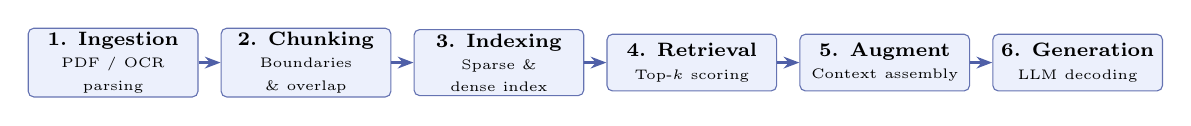
\begin{tikzpicture}[
    stage/.style={draw=primaryblue!70,fill=tableheader,rounded corners=2pt,text width=2.05cm,
      minimum height=0.72cm,align=center,font=\scriptsize,inner sep=1.5pt},
    flow/.style={-{Stealth[length=2mm]},thick,draw=primaryblue!80}
  ]
    \node[stage] (s1) at (0,0) {\textbf{1. Ingestion}\\\tiny PDF / OCR parsing};
    \node[stage] (s2) at (2.45,0) {\textbf{2. Chunking}\\\tiny Boundaries \& overlap};
    \node[stage] (s3) at (4.9,0) {\textbf{3. Indexing}\\\tiny Sparse \& dense index};
    \node[stage] (s4) at (7.35,0) {\textbf{4. Retrieval}\\\tiny Top-$k$ scoring};
    \node[stage] (s5) at (9.8,0) {\textbf{5. Augment}\\\tiny Context assembly};
    \node[stage] (s6) at (12.25,0) {\textbf{6. Generation}\\\tiny LLM decoding};
    
    \draw[flow] (s1) -- (s2);
    \draw[flow] (s2) -- (s3);
    \draw[flow] (s3) -- (s4);
    \draw[flow] (s4) -- (s5);
    \draw[flow] (s5) -- (s6);
  \end{tikzpicture}

  \vspace{0.25cm}
  \begin{itemize}
    \setlength{\itemsep}{0.25cm}
    \item \textbf{Pre-Retrieval Failure Points:} OCR noise on scanned documents; premature text splits detaching qualifying exceptions from primary articles.
    \item \textbf{Retrieval Failure Points:} False negative omissions (gold threshold clauses rank outside top-$k$); lexical distractor confusion.
    \item \textbf{Post-Retrieval Failure Points:} Context distraction; condition omission; table column misreading; failure to produce verifiable citation IDs.
  \end{itemize}

  \source{Adapted from Lewis et al. (2020), Figure 1; CS420 S07 Report \S4.2, Figure 1.}
\end{frame}

% Slide 06: Probabilistic Modeling: Sequence vs. Token
\begin{frame}{Probabilistic Modeling: Sequence vs.\ Token}
  \vspace{-0.1cm}
  {\footnotesize\textbf{1. RAG-Sequence (Sequence-Level Marginalization):}\par}
  \vspace{-4pt}
  \[
    p_{\mathrm{Seq}}(y \mid x) \approx \sum_{z \in \mathrm{top-}k} p_\eta(z \mid x) \prod_{i=1}^{T} p_\theta(y_i \mid x, z, y_{<i})
  \]
  \vspace{-4pt}
  {\footnotesize\textbf{2. RAG-Token (Token-Level Step Marginalization):}\par}
  \vspace{-4pt}
  \[
    p_{\mathrm{Tok}}(y \mid x) \approx \prod_{i=1}^{T} \left[ \sum_{z \in \mathrm{top-}k} p_\eta(z \mid x) p_\theta(y_i \mid x, z, y_{<i}) \right]
  \]

  \begin{itemize}
    \setlength{\itemsep}{0.12cm}
    \item \textbf{Latent Passage ($z$):} Retrieved documents act as latent variables marginalized across top-$k$ candidates.
    \item \textbf{Sequence Formulation:} Generates entire response $y$ from a single document $z$; preserves topic coherence.
    \item \textbf{Token Formulation:} Dynamically switches documents across tokens; ideal for synthesizing multi-source facts.
    \item \textbf{Variables:} $x$: query; $y_{<i}$: generated prefix; $\eta, \theta$: retriever/generator parameters; $p \in [0, 1]$.
  \end{itemize}

  \source{Lewis et al. (NeurIPS 2020), \S2.1, Equations (1)--(2).}
\end{frame}

% Slide 07: Worked Numerical Example (k=2, T=2)
\begin{frame}{Worked Numerical Example ($k=2, T=2$)}
  \vspace{-0.1cm}
  \begin{table}[H]
    \centering
    \footnotesize
    \renewcommand{\arraystretch}{1.2}
    \begin{tabularx}{\textwidth}{>{\bfseries\raggedright\arraybackslash}p{2.5cm} *{3}{>{\centering\arraybackslash}X}}
      \toprule
      \rowcolor{tableheader}
      Passage ($z$) & Retriever Weight $p_\eta(z \mid x)$ & $p_\theta(a \mid x, z)$ & $p_\theta(b \mid x, z, a)$ \\
      \midrule
      $z_1$ & 0.70 & 0.80 & 0.90 \\
      $z_2$ & 0.30 & 0.40 & 0.20 \\
      \bottomrule
    \end{tabularx}
  \end{table}

  \vspace{0.1cm}
  \begin{itemize}
    \setlength{\itemsep}{0.2cm}
    \item \textbf{RAG-Sequence Calculation:}
      \[
        p_{\mathrm{Seq}} = 0.70 \times (0.80 \times 0.90) + 0.30 \times (0.40 \times 0.20) = 0.5040 + 0.0240 = \mathbf{0.5280}
      \]
    \item \textbf{RAG-Token Calculation:}
      \[
        p_{\mathrm{Tok}} = (0.70 \times 0.80 + 0.30 \times 0.40) \times (0.70 \times 0.90 + 0.30 \times 0.20) = 0.6800 \times 0.6900 = \mathbf{0.4692}
      \]
    \item \textbf{Operator Inversion:} The discrepancy ($0.5280$ vs.\ $0.4692$) reflects the non-commutativity of $\sum$ and $\prod$.
    \item \textbf{Implementation Distinction:} Modern instruction-tuned QA (e.g., Qwen) performs prompt conditioning rather than explicit marginalization.
  \end{itemize}

  \source{CS420 S07 Report \S3.2, Table 1. Probabilities parameterized to demonstrate mathematical formulation.}
\end{frame}


% --- PART 2: HCMUS Corpus & Retrieval Experiments (Speaker 2: Lê Huy, 05:00 - 10:00) ---
% Slide 08: Experimental Corpus: HCMUS Regulations
\begin{frame}{Experimental Corpus: HCMUS Regulatory Documents}
  \vspace{-0.1cm}
  \begin{table}[H]
    \centering
    \footnotesize
    \renewcommand{\arraystretch}{1.15}
    \begin{tabularx}{\textwidth}{>{\bfseries}l X l c}
      \toprule
      \rowcolor{tableheader}
      ID & Regulatory Document Title and Reference & Scope & Pages \\
      \midrule
      D01 & Undergraduate Academic Regulations 2026 (Dec.\ 3087/QĐ-KHTN) & Academic Rules & 21 \\
      D02 & Student Conduct Assessment 2020 \& Amendment 2023 & Conduct Scoring & 16 \\
      D03 & Tuition Fee Rates AY 2026--2027 (Dec.\ 3317/QĐ-KHTN) & Fees (K2022+) & 5 \\
      D04 & Foreign Language Graduation Standards (Dec.\ 2464/QĐ-KHTN) & Exit Standards & 9 \\
      \midrule
      \rowcolor{tablehighlight}
      Total & Authoritative four-document regulatory snapshot & PDF Corpus & \textbf{51} \\
      \bottomrule
    \end{tabularx}
  \end{table}

  \vspace{0.1cm}
  \begin{itemize}
    \setlength{\itemsep}{0.2cm}
    \item \textbf{Corpus Scale:} 51 pages segmented into 80 parent sections and 162 chunks under an 800-token ceiling (\texttt{cl100k\_base}).
    \item \textbf{Evaluation Benchmark:} 20 administrative queries mapped to 30 gold evidence groups (held out from indexing).
    \item \textbf{Metadata Preservation:} Articles, PDF page numbers, cohort scopes, and table footnotes injected into chunk headers.
    \item \textbf{Scope Distinction:} Exceeds standard 5--10 page guideline to test real-world administrative cross-referencing.
  \end{itemize}

  \source{CS420 S07 Report \S4.1, Table 2. Verified against official HCMUS portals (commit 3bb5f3a).}
\end{frame}

% Slide 09: Retrieval Configurations & Evaluation Protocol
\begin{frame}{Retrieval Configurations \& Evaluation Protocol}
  \vspace{-0.1cm}
  \begin{table}[H]
    \centering
    \footnotesize
    \renewcommand{\arraystretch}{1.2}
    \begin{tabularx}{\textwidth}{>{\bfseries}l l X l}
      \toprule
      \rowcolor{tableheader}
      Retriever & Type & Representation & Hyperparameters \\
      \midrule
      TF-IDF & Sparse Lexical & Unigram + bigram frequencies & Sublinear TF, cosine distance \\
      BM25 & Sparse Lexical & Term frequency saturation \& length penalty & Vietnamese tokens, $k_1=1.5, b=0.75$ \\
      BGE-M3 & Dense Neural & 1024-dim multilingual dense embeddings & Normalized vectors, cosine similarity \\
      \bottomrule
    \end{tabularx}
  \end{table}

  \vspace{0.1cm}
  \begin{itemize}
    \setlength{\itemsep}{0.2cm}
    \item \textbf{Evaluation Metrics (Macro-averaged across 20 queries, 30 gold evidence groups):}
      \begin{itemize}
        \item \textbf{Evidence Recall@$k$:} Fraction of necessary gold evidence groups retrieved ($r/m$).
        \item \textbf{Hit Rate@$k$:} Binary indicator if at least one gold evidence group is found ($r \ge 1$).
        \item \textbf{All Evidence Hit@$k$:} Binary indicator if all gold evidence groups are retrieved ($r = m$).
        \item \textbf{MRR@$k$:} Reciprocal rank of the first relevant evidence chunk (0 if not in top-$k$).
      \end{itemize}
    \item \textbf{Benchmark Cut-offs:} Evaluated at $k \in \{1, 3, 5\}$ to compare early precision vs.\ multi-hop recall.
  \end{itemize}

  \source{CS420 S07 Report \S4.1; Retrieval evaluation scripts at commit \commitlink{5771d80}.}
\end{frame}

% Slide 10: Experiment 1: Retrieval Performance
\begin{frame}{Experiment 1: Retrieval Performance}
  \vspace{-0.1cm}
  \begin{table}[H]
    \centering
    \footnotesize
    \renewcommand{\arraystretch}{1.2}
    \begin{tabularx}{\textwidth}{>{\bfseries\raggedright\arraybackslash}p{2.2cm} *{6}{>{\centering\arraybackslash}X}}
      \toprule
      \rowcolor{tableheader}
      Retriever & Recall@1 & Recall@3 & Recall@5 & Hit@5 & All Evidence@5 & MRR@5 \\
      \midrule
      TF-IDF & 70.83\% & 82.50\% & 82.50\% & 90.00\% & 15/20 & 0.8250 \\
      BM25 & \textbf{80.00\%} & \textbf{84.17\%} & 84.17\% & 90.00\% & \textbf{16/20} & \textbf{0.8667} \\
      BGE-M3 & 65.00\% & 81.67\% & \textbf{89.17\%} & \textbf{95.00\%} & \textbf{16/20} & 0.7867 \\
      \bottomrule
    \end{tabularx}
  \end{table}

  \vspace{0.1cm}
  \begin{itemize}
    \setlength{\itemsep}{0.2cm}
    \item \textbf{Early Precision (BM25):} BM25 dominates top-1 ranking (Recall@1 = 80.00\%) via exact lexical matching of regulatory terms.
    \item \textbf{High-Cutoff Coverage (BGE-M3):} Dense embeddings lead at $k=5$ (Recall@5 = 89.17\%, Hit@5 = 95.00\%) by capturing semantic paraphrases.
    \item \textbf{Plateau Effect:} Lexical methods saturate at $k=3$, whereas BGE-M3 gains +7.50 percentage points expanding from $k=3$ to $k=5$.
    \item \textbf{Crucial Takeaway:} \textcolor{alertred}{\textbf{Hit@5 = 95.00\% does NOT imply 95\% answer accuracy!}} Downstream generation bottlenecks persist.
  \end{itemize}

  \source{CS420 S07 Report \S5, Table 4. Evaluated on 20 queries, 30 gold evidence groups (commit \commitlink{5771d80}).}
\end{frame}

% Slide 11: Worked Example (Q01): Top-5 Candidate Chunks
\begin{frame}{Worked Example (Q01): Top-5 Candidate Chunks}
  \vspace{-0.1cm}
  {\footnotesize\textbf{Benchmark Query (Q01):} \emph{According to the 2026 Academic Regulations, how does a prerequisite course differ from a pre-learning course?}}
  \vspace{0.15cm}

  \begin{table}[H]
    \centering
    \scriptsize
    \renewcommand{\arraystretch}{1.15}
    \begin{tabularx}{\textwidth}{c l c c X}
      \toprule
      \rowcolor{tableheader}
      Rank & Chunk Identifier & Cosine & Page & Content Summary and Regulatory Scope \\
      \midrule
      \rowcolor{tablehighlight}
      \textbf{1} & \chunkid{D01\_regulation\_article\_3\_03} & \textbf{0.6271} & 4 & \textbf{Gold Evidence:} Article 3, Clause 3(c) (Both definitions) \\
      2 & \chunkid{D01\_regulation\_article\_27\_01} & 0.5813 & 21 & Article 27: Transitional clauses for earlier cohorts \\
      3 & \chunkid{D01\_regulation\_article\_3\_02} & 0.5704 & 3 & Article 3, Clause 2: Elective and general course definitions \\
      4 & \chunkid{D01\_regulation\_article\_6\_02} & 0.5643 & 7 & Article 6: Semester scheduling and course limits \\
      5 & \chunkid{D01\_regulation\_article\_18\_02} & 0.5540 & 16 & Article 18: Credit exemptions and transfer guidelines \\
      \bottomrule
    \end{tabularx}
  \end{table}

  \vspace{0.05cm}
  \begin{itemize}
    \setlength{\itemsep}{0.18cm}
    \item \textbf{Successful Top-1 Alignment:} Rank-1 passage provides 100\% of required gold evidence for both course concepts.
    \item \textbf{Crucial Regulatory Distinction:} Prerequisite requires ``passing'' the exam; pre-learning only requires ``completing the coursework''.
    \item \textbf{Distractor Risk:} Ranks 2--5 introduce adjacent credit/scheduling rules that risk inducing model confusion.
  \end{itemize}

  \source{CS420 S07 Report \S4.2, Table 3. Dense ranking log from \texttt{retrieval\_hits.json}.}
\end{frame}

% Slide 12: Worked Example (Q01): Grounded vs. Baseline Output
\begin{frame}{Worked Example (Q01): Grounded vs.\ Baseline Output}
  \vspace{-0.1cm}
  \begin{table}[H]
    \centering
    \footnotesize
    \renewcommand{\arraystretch}{1.2}
    \begin{tabularx}{\textwidth}{>{\bfseries}l c X}
      \toprule
      \rowcolor{tableheader}
      Configuration & Score & Generated Response Content \& Attribution \\
      \midrule
      Baseline (No RAG) & 0 / 2 & Hallucinates generic academic progression; falsely claims both course types require passing grades; lacks any regulatory citation. \\
      \midrule
      \rowcolor{tablehighlight}
      Grounded RAG (BGE-M3) & \textbf{2 / 2} & Correctly states prerequisite requires \textbf{``passing''} (thi đạt), while pre-learning only requires \textbf{``completing the study process''}. \newline {\scriptsize[\chunkid{D01\_regulation\_article\_3\_03}]$^*$} \\
      \bottomrule
    \end{tabularx}
  \end{table}

  \vspace{0.1cm}
  \begin{itemize}
    \setlength{\itemsep}{0.2cm}
    \item \textbf{Prompt Augmentation:} Context injected under structured \texttt{SOURCES} block with chunk IDs, article titles, and page numbers.
    \item \textbf{Factual Grounding Contrast:} Parametric memory guesses incorrectly; RAG context enables precise legal differentiation.
    \item \textbf{$^*$Human Attribution Caveat:} Qwen generated the correct text but failed to emit the citation ID; the reference tag was verified and added post-hoc by human auditors.
  \end{itemize}

  \source{CS420 S07 Report \S4.2; Task 6 answer comparison logs. $^*$Citation verified and appended during human audit.}
\end{frame}


% --- PART 3: Answer Quality, Failure Analysis & Verification (Speaker 3: Tuấn Lĩnh, 10:00 - 15:00) ---
% Slide 13: Experiment 2: 4-Way Answer Quality
\begin{frame}{Experiment 2: 4-Way Answer Quality}
  \vspace{-0.1cm}
  \begin{table}[H]
    \centering
    \footnotesize
    \renewcommand{\arraystretch}{1.2}
    \begin{tabularx}{\textwidth}{>{\bfseries\raggedright\arraybackslash}p{3.4cm} *{5}{>{\centering\arraybackslash}X}}
      \toprule
      \rowcolor{tableheader}
      Configuration & Fully Correct & Partial & Incorrect & Unsupported & Valid Citations \\
      \midrule
      Baseline (No RAG) & 0/20 (0.0\%) & 3/20 (15.0\%) & 17/20 (85.0\%) & 15/20 (75.0\%) & 0/20 (0.0\%) \\
      RAG (TF-IDF) & \textbf{10/20 (50.0\%)} & 5/20 (25.0\%) & 5/20 (25.0\%) & 8/20 (40.0\%) & 0/20 (0.0\%) \\
      RAG (BM25) & 9/20 (45.0\%) & 6/20 (30.0\%) & 5/20 (25.0\%) & 7/20 (35.0\%) & 0/20 (0.0\%) \\
      RAG (BGE-M3) & \textbf{10/20 (50.0\%)} & 6/20 (30.0\%) & 4/20 (20.0\%) & \textbf{6/20 (30.0\%)} & 0/20 (0.0\%) \\
      \bottomrule
    \end{tabularx}
  \end{table}

  \vspace{0.1cm}
  {\centering\large\textbf{\textcolor{primaryblue}{+45.0 to +50.0 pp accuracy gain over unaugmented baseline (0\% $\to$ 50\%)}}\par}
  \vspace{0.1cm}

  \begin{itemize}
    \setlength{\itemsep}{0.18cm}
    \item \textbf{Recall $\neq$ Accuracy Bottleneck:} Despite higher Evidence Recall@5 (89.17\%), BGE-M3 ties with TF-IDF at 50\% accuracy.
    \item \textbf{Significant Hallucination Drop:} Unsupported claims decrease from 75\% in baseline to 30\% in BGE-M3 and 35\% in BM25.
    \item \textbf{Universal Citation Blindness:} All 60 RAG answers omitted formal citation tags despite explicit prompt constraints.
  \end{itemize}

  \source{CS420 S07 Report \S5, Table 5. Evaluated on Qwen2.5-1.5B-Instruct across 80 completions (commit \commitlink{3bb5f3a}).}
\end{frame}

% Slide 14: Empirical Failure Archetypes
\begin{frame}{Empirical Failure Modes: 5 Representative Cases}
  \vspace{-0.1cm}
  \begin{table}[H]
    \centering
    \scriptsize
    \renewcommand{\arraystretch}{1.15}
    \begin{tabularx}{\textwidth}{c X X}
      \toprule
      \rowcolor{tableheader}
      Query & Observed Prompt and Generation Behavior & Root Cause and Remediation Stage \\
      \midrule
      \textbf{Q07} & Top-5 misses the 65--79 score band chunk. BGE-M3 fabricates ``Average 50 points'' for a 68-point score. & \textbf{Retrieval Omission:} Gold threshold missing; model guesses parametrically. \\
      \textbf{Q01} & Correct definition ranks 1. TF-IDF/BM25 rank English prerequisite at rank 2, derailing output focus. & \textbf{Distractor Interference:} Lexical match confuses cross-attention context. \\
      \textbf{Q05} & Model receives Article 19 but asserts credit completion alone suffices for graduation. & \textbf{Condition Pruning:} Generator overlooks secondary administrative rules. \\
      \textbf{Q13} & All retrievers capture tuition table. Model reads column C1 (488k) instead of C5 (1,014k vs.\ 974k). & \textbf{Tabular Misalignment:} 1.5B LLM struggles with row-column intersections. \\
      \textbf{Q19} & Model captures valid deadlines but fabricates a non-existent decision suffix identifier. & \textbf{Metadata Hallucination:} Generates plausible-sounding official numbers. \\
      \bottomrule
    \end{tabularx}
  \end{table}

  \vspace{0.05cm}
  \begin{itemize}
    \setlength{\itemsep}{0.15cm}
    \item \textbf{Comprehensive Distribution:} Failures occur across retrieval (Q07, Q01), reasoning (Q05), tables (Q13), and citations (Q19).
    \item \textbf{High Risk of Structured Data:} Multi-column tables and multi-condition checklists require specialized extraction pipelines.
  \end{itemize}

  \source{CS420 S07 Report \S6, Table 6. Case analysis from 80-answer generation logs (commit \commitlink{3bb5f3a}).}
\end{frame}

% Slide 15: Discussion: Does RAG Eliminate Hallucinations?
\begin{frame}{Discussion: Does RAG Eliminate Hallucinations?}
  \vspace{0.1cm}
  % Part 1: Core Research Question & Immediate Finding
  {\Large\textbf{Does providing external documents eliminate hallucinations?}}
  \vspace{0.25cm}

  {\LARGE\textbf{\textcolor{alertred}{NO.}}\quad\normalsize\textbf{RAG transforms the nature and origin of hallucinations.}}
  \vspace{0.35cm}

  \pause
  % Part 2: Paradigm Shift & Grounding Fallacy
  \begin{itemize}
    \setlength{\itemsep}{0.22cm}
    \item \textbf{Paradigm Shift in Errors:} RAG resolves the parametric knowledge deficit (jumping from 0\% to 50\% accuracy), but introduces pipeline-dependent vulnerabilities.
    \item \textbf{The Grounding Fallacy:} Supplying relevant documents is a \emph{necessary} condition, but \emph{not a sufficient} condition to guarantee factual truthfulness.
  \end{itemize}

  \pause
  \vspace{0.1cm}
  % Part 3: Cascading Pipeline Errors & Theoretical Literature
  \begin{itemize}
    \setlength{\itemsep}{0.22cm}
    \item \textbf{Cascading Pipeline Errors:} Hallucinations now emerge from retrieval omissions, adjacent distractors, condition pruning, and tabular distortion.
    \item \textbf{Literature Corroboration:} Aligns with Schneider (2024, GenXAI) and Niu et al.\ (ACL 2024, RAGTruth): LLMs frequently assert ungrounded claims despite prompt grounding.
  \end{itemize}

  \source{Schneider (2024), GenXAI, \S1--\S2; Niu et al. (ACL 2024), RAGTruth; CS420 S07 Report \S1, \S6.}
\end{frame}

% Slide 16: Limitations & Applicability Boundaries
\begin{frame}{Limitations \& Applicability Boundaries}
  \vspace{0.1cm}
  \begin{itemize}
    \setlength{\itemsep}{0.28cm}
    \item \textbf{Benchmark Sample Size:} 20 curated administrative queries; a single outcome change shifts performance by 5.0 percentage points (requires cautious statistical interpretation).
    \item \textbf{Corpus Scope:} 51 pages across 4 documents from a single university; 29 pages OCR-processed without complete token-level human audit.
    \item \textbf{Evaluation Methodology:} Correctness scores were assigned via automated GPT-based qualitative review; double-blind human cross-annotation remains pending.
    \item \textbf{Generator Scale:} Evaluated on a frozen 1.5B instruction-tuned model (\texttt{Qwen2.5-1.5B-Instruct}); larger models (7B/72B) may better interpret complex tables.
    \item \textbf{Inference Context Overhead:} Top-5 RAG increases prompt tokens from 236 to 2,749--3,205 tokens ($\approx 12\times$ latency and API cost increase).
  \end{itemize}

  \source{CS420 S07 Report \S7. Limitations documented in accordance with seminar evaluation standards.}
\end{frame}

% Slide 17: Proposed Improvements: Verification & Maintenance
\begin{frame}{Proposed Improvements: Verification \& Maintenance}
  \vspace{-0.1cm}
  \begin{block}{1. Post-Generation Verification Loop (Schneider, 2024 --- GenXAI)}
    \begin{itemize}
      \setlength{\itemsep}{0.12cm}
      \item \textbf{Atomic Claim Decomposition:} Deconstruct generated answers into verifiable tuples:
        \[
          \langle\text{Claim},\ \text{Applicable Cohort},\ \text{Chunk ID},\ \text{Verbatim Quote}\rangle
        \]
      \item \textbf{Natural Language Inference (NLI) Gate:} Automatically audit entailment between claim and quote; trigger safe abstention (``Insufficient information'') if ungrounded.
    \end{itemize}
  \end{block}

  \begin{block}{2. Tabular Structuring \& Regulatory Maintenance}
    \begin{itemize}
      \setlength{\itemsep}{0.12cm}
      \item \textbf{Structured Table Parsing:} Convert dense multi-column tuition matrices into explicit key-value schemas to eliminate column misalignment (as observed in Q13).
      \item \textbf{Versioned Corpus Registry:} Track circulars by decision number, effective date, and SHA-256 hash; execute automated diffs to retire obsolete regulatory chunks.
    \end{itemize}
  \end{block}

  \source{Schneider (2024), GenXAI, \S3.3; CS420 S07 Report \S6. Proposed architectural improvements.}
\end{frame}

% Slide 18: Conclusions & Core Takeaways
\begin{frame}{Conclusions \& Core Takeaways}
  \vspace{0.1cm}
  \begin{itemize}
    \setlength{\itemsep}{0.25cm}
    \item \textbf{Substantial Accuracy Lift:} RAG elevates core factual correctness from 0\% in an unaugmented baseline to 45--50\% on complex administrative regulations.
    \item \textbf{Complementary Retrieval Roles:} BM25 delivers highest top-1 precision (Recall@1 = 80.00\%); BGE-M3 provides greatest aggregate coverage (Recall@5 = 89.17\%).
    \item \textbf{The Verification Imperative:} High recall ($\text{Hit@5} = 95\%$) is insufficient. Generators omit conditions, confuse tables, and fail at citation IDs.
    \item \textbf{Core Takeaway:} Curing hallucinations requires treating retrieval, structured parsing, and post-generation claim verification as an integrated pipeline.
  \end{itemize}

  \vfill
  \begin{center}
    {\large\bfseries\color{primaryblue} External documents ground LLMs, but only rigorous verification ensures reliability.}
  \end{center}

  \source{CS420 S07 Seminar Report, Faculty of Information Technology, HCMUS (2026).}
\end{frame}

% Slide 19: References
\begin{frame}{Key References}
  \vspace{-0.1cm}
  \begin{itemize}
    \footnotesize
    \setlength{\itemsep}{0.2cm}
    \item \textbf{Lewis, P. et al.\ (2020).} Retrieval-Augmented Generation for Knowledge-Intensive NLP Tasks. \emph{Advances in Neural Information Processing Systems (NeurIPS)}, 33, 9459--9474.
    \item \textbf{Schneider, J.\ (2024).} Explainable Generative AI (GenXAI): A survey, conceptualization, and research agenda. \emph{Artificial Intelligence Review}, 57, 289.
    \item \textbf{Chen, J. et al.\ (2024).} M3-Embedding: Multi-Linguality, Multi-Functionality, Multi-Granularity Text Embeddings Through Self-Knowledge Distillation. \emph{arXiv:2402.03216}.
    \item \textbf{Qwen Team (2024).} Qwen2.5 Technical Report. \emph{arXiv:2412.15115}.
    \item \textbf{VNU-HCM University of Science (2020--2026).} Decisions 3087/QĐ-KHTN (Academic), 3317/QĐ-KHTN (Tuition), 2464/QĐ-KHTN (Language), and Student Conduct 2020/2023.
    \item \textbf{Project Artifacts \& Codebase:} \url{https://github.com/namkiet/CS420_SeminarRAG}
  \end{itemize}

  \source{All references verified and archived in repository directory \texttt{docs/} and \texttt{report/}.}
\end{frame}

% Slide 20: Thank You & Q&A
\begin{frame}[plain]
  \vspace{1.5cm}
  \begin{center}
    {\Huge\bfseries\textcolor{primaryblue}{Thank you for listening!}\par}
    
    \vspace{0.8cm}
    {\LARGE\textbf{Any questions?}\par}
  \end{center}
\end{frame}


\end{document}
